\documentclass[10pt]{article}
\usepackage[margin=0.7in]{geometry}
\usepackage[T1]{fontenc}
\usepackage{lmodern,graphicx,booktabs,array,hyperref,fancyhdr,amsmath}
\hypersetup{colorlinks=true,urlcolor=blue}
\pagestyle{fancy}\fancyhf{}\lhead{Classical prime-field ECDLP counter audit}\rhead{23 November 2026}\cfoot{Unsigned producer claims --- \thepage}
\setlength{\headheight}{14pt}\setlength{\parindent}{0pt}\setlength{\parskip}{5pt}
\begin{document}
{\Large\bfseries Finite inherited precision and composed sharp bound}

The exact integer precision recurrence now has a kernel-checked finite-history
bound and a formal composition with the shared sharp endpoint. Three history
statements and eight numeric instance controls compile; the local PCC proof
verifier passes. Claims \texttt{PCC-20261123-dc026e} and
\texttt{PCC-20261123-8bf465} remain unsigned and unverified in ledger standing.

Write $C(P,M,u,a,i)=P+8\lceil3M/u\rceil2^{a-i}+8M(a+1)$ for
the shared Nat expression, with natural subtraction. For supplied finite arrays,
assume $M_0\le s$, $p_0\le s$, and, for every $k<d$,
\[
8M_{k+1}\le M_k,\quad0<u_k\le M_k,\quad a_k\le A,
\qquad p_{k+1}=C(p_k,M_k,u_k,a_k,i_k).
\]
Then the new history theorem derives
\[
\boxed{p_d\le81s2^A}.
\]
Existing Mathlib finite-index comparison and geometric-sum laws give
$\sum_{k<d}M_k\le2s$. The shared increment law gives an accumulated
increment of at most $80s2^A$. The exact Nat recurrence telescopes, and
$p_0\le s\le s2^A$ supplies the last term. No inherited-budget conclusion is
assumed as a premise, and no infinite positive shrinking path is assumed.

At the next call put $a=A+2u_d$ and $D=2^{a-i_d}$, supplying its exact next
precision formula. If also
\[
u_d\le M_d,\quad i_d<u_d,\quad s\le M_dq,
\]
\[
81qu_d\le2^{u_d+1},\qquad
8u_d(A+2u_d+1)\le2^{A+u_d+1},
\]
the composed theorem proves $u_dp_{d+1}\le34M_dD$ by deriving the inherited
budget and applying the shared scalar endpoint.

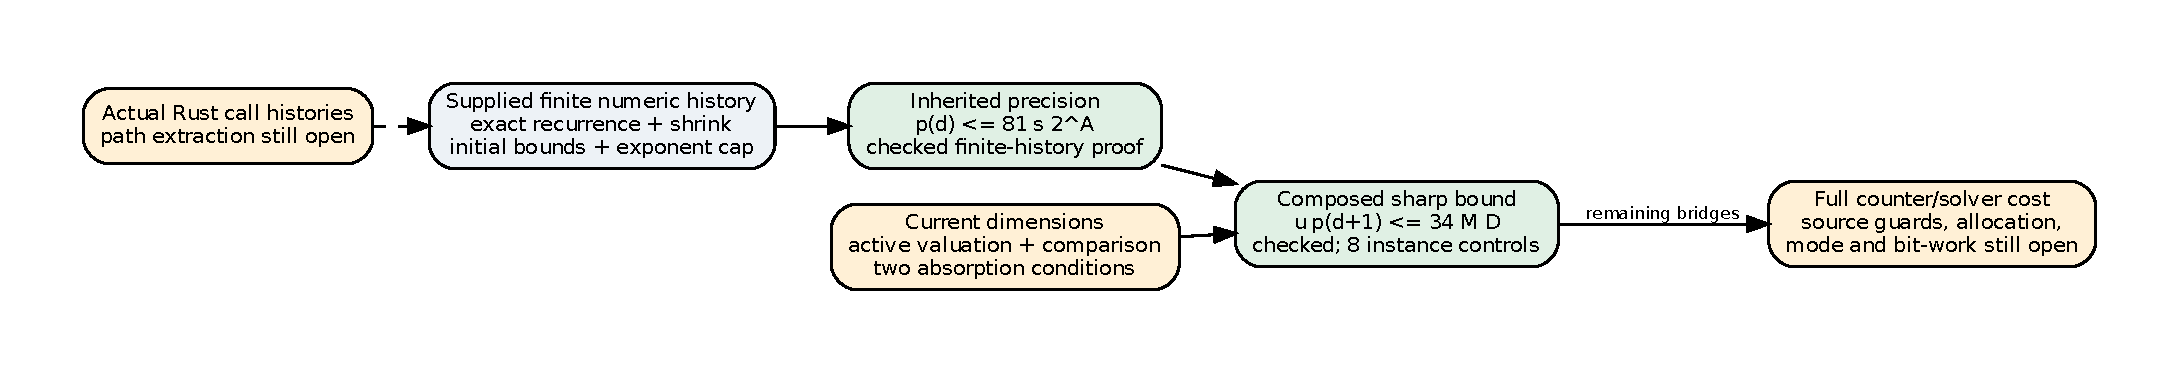
\includegraphics[width=\linewidth]{history-map.pdf}

\textbf{Source and scope.} Primary Appendix D.11: openai/math42907c9e,
TeX blob51ba54ef. Shared Std model: crypto-lean3e47fb77, PR35. Native
precision/shrink/subdivision expressions: crypto main816f9c3a, PR4996.
$M$ is a network edge count and $p$ a bit precision, not the field modulus.
These are numeric-history bounds. Actual successful Rust path extraction,
source-guard absorption and full counter/solver cost remain separate.

\newpage
{\Large\bfseries Controls, initial normalization and provenance}

\begin{tabular}{@{}p{0.27\linewidth}p{0.68\linewidth}@{}}\toprule
Control & Result and scope \\\midrule
Empty history & Initial budget with zero increments.\\
Two-step history & Exact increments, edges64,8,1, bounded prior exponents.\\
Composed endpoint & History plus explicit current dimension conditions.\\
Delete initial precision & Keeps other named premises; raised starting precision violates81.\\
Delete root edge bound & Keeps other named premises; edges decouple from size.\\
Delete shrink & Constant edges and exact repeated increments violate81.\\
Delete exponent cap & Earlier exponent exceeds the supplied common cap.\\
Delete recurrence & Dimensions alone leave final precision unconstrained.\\\bottomrule
\end{tabular}

These are eight distinct numeric controls, not solver runs. The composed positive
has synthetic parameters, including an increasing scale and $M_0=E$; it is not
an extracted native path. The actual subdivided native root has $M_0=s=2E$,
with initial precision $E+1\le2E$ for nonempty $E$. The helper's first
conjunct $E\le2E$ concerns original unsubdivided edges. General $p_0\le Cs$
changes the81 coefficient. Deletion controls do not make every sufficient
condition pointwise necessary.

\textbf{Axioms and dependencies.} All eleven axiom queries pass. The history,
normalization, composition and positive controls use only standard
\texttt{propext}, \texttt{Classical.choice}, \texttt{Quot.sound}; the five
deletion controls use the first and last. Original Lean4.35.0 and exact
Mathlib56a00585 are used. The imported shared module is Std-only; crypto-lean's
different Mathlib pin is not substituted or qualified by this instance.
No native algorithm, dependency pin, proof gate or trust list changed.

\textbf{Review.} A separate read-only reviewer found no blocking algebra or
control issue in the frozen source through gate18. Its source/initialization
limits are retained. This review is unsigned and does not independently run
Lean or attest execution. Committed-artifact binding is a separate addendum.

\textbf{Failures and isolation.} A cast-name/normalization error is retained
before correction. Gate19 reached the unchanged physical stop and produced no
verdict. Attempt20 passed proof checks but began one second before gate19
finished; it is not accepted as isolated qualification. Later outer
launches acquire the shared worker lock. Malformed proof registrationf665ec
fails locally and remains unchanged, distinct from corrected claimdc026e.
Isolated phase22 passes all builds/axioms and both gates. Its controls audit
has9declarations: eight named controls plus the shared defining equation,
with zero failing/trusted entries. Requalification adds no logical instances.
Raw terminal outcomes are retained in checks.

\textbf{Cache and resource boundary.}455 needed private dependency files were
restored and rehashed. A further bounded external-cache subset outside the
inventoried import closure was preserved losslessly before compacting duplicate
uncompressed copies. Owned research, proof checkpoints, binaries and earlier
handoffs remain intact. Limits stay one worker,600seconds per phase and
15,032,385,536bytes whole-cgroup. No performance inference or additional
capacity/spend follows; Amazon S3 storage remains excluded.

\textbf{Remaining work.} Extract actual paths and cumulative parameters, prove
source absorption, then packet/mode, construction precision, allocation,
rational-width and entry bit-work bridges. Reconcile the optimized baseline
and complete the frozen84-case/larger solver comparison separately. No solver,
asymptotic or novelty conclusion follows from this component proof.

\url{https://github.com/isogeny-labs/crypto/pull/4996}\quad
\url{https://github.com/aburan28/crypto-lean/pull/35}
\end{document}
